\section{Aufbau und Durchführung}

\begin{figure}[h!tbp]
	\centering
	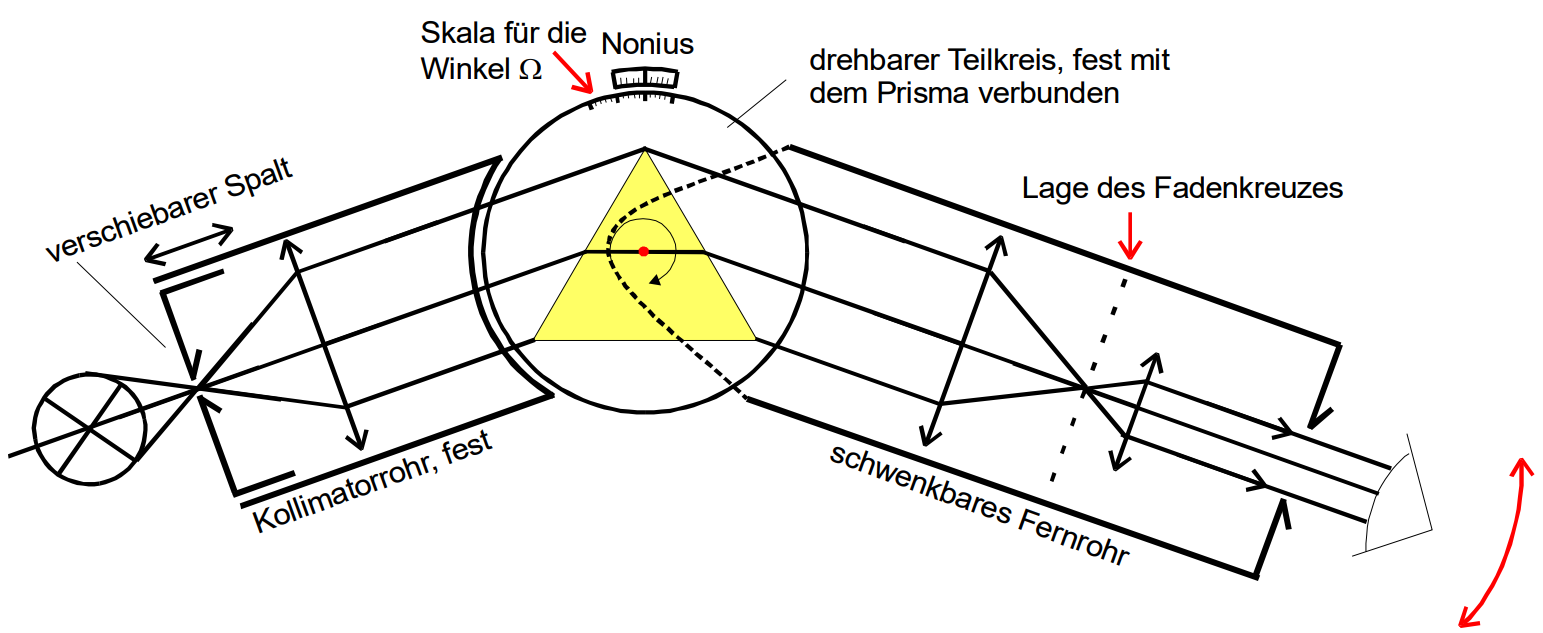
\includegraphics[width=0.7\linewidth]{aufbau}
	\caption{Aufbau des Prismen-Spektralapparates, \cite[9]{anleitungV402}.}
	\label{fig:aufbau}
\end{figure}

Zur Apparatur gehört eine Heliumlampe, dessen Licht auf ein Glasprisma fällt, in dem es, sofern das Licht unter einem Winkel auftrifft, zweimal gebrochen wird. Mithilfe eines schwenkbaren Fernrohres können dann unter bestimmten Winkeln Spaltbilder 
beobachtet werden, die eingestellten Winkel werden dann an der angebrachten Scheibe abgelesen.

Im ersten Versuchsteil soll der Winkel $\varphi$ zwischen den brechenden Prismenoberflächen bestimmt werden. Hierzu wird das Prisma so ausgerichtet, dass eine Spitze zur He-Lampe zeigt. Das Fernrohr wird dann auf die reflektierten Strahlen des Lichts
ausgerichtet und die Winkel $\varphi_{\text{l}}$ und $\varphi_{\text{r}}$, wie in Abbildung \ref{fig:aufbau} zu sehen, auf der rechten und linken Seite des Prismas abgelesen.
Der Winkel $\varphi$ berechnet sich nun zu:

\begin{equation}
\label{eq:varphi}
\varphi = \frac{1}{2} (\varphi_{\text{r}} - \varphi_{\text{l}}).
\end{equation}

\begin{figure}[h!tbp]
	\centering
	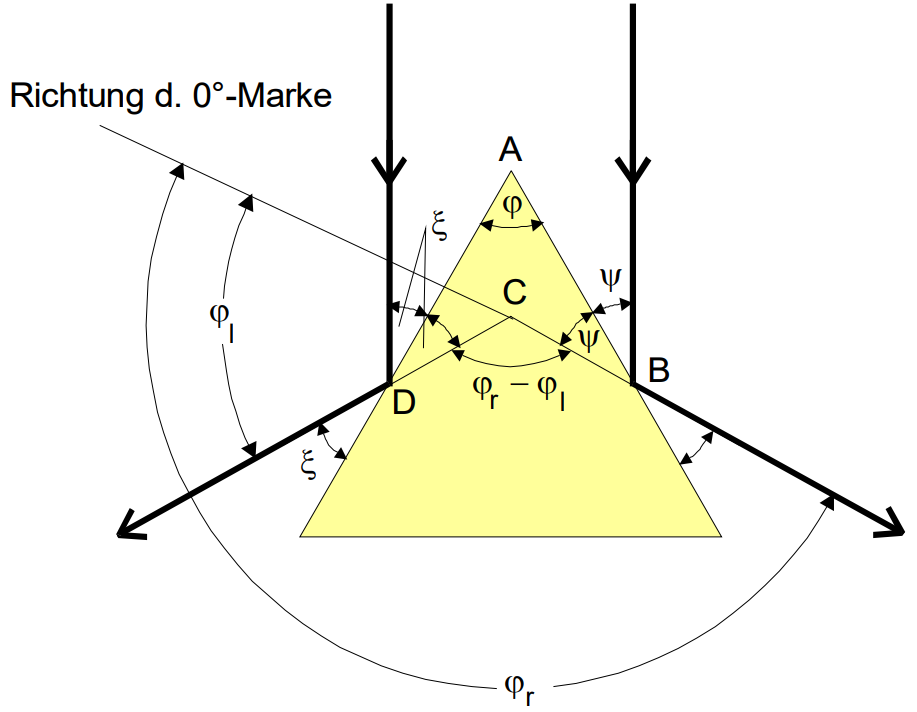
\includegraphics[width=0.7\linewidth]{phi}
	\caption{Skizze zur Bestimmung des Winkels $\varphi$, \cite[11]{anleitungV402}.}
	\label{fig:phi}
\end{figure}

Im zweiten Teil des Versuchs werden die Brechungswinkel $\eta_{\text{i}}$ für sichtbaren Linien des Helium-Sprektrums bestimmt, wofür ein symmetrischer Strahlengang notwendig ist. Das Prisma wird so gedreht, bis das Spaltbild mit dem reflektierten 
Strahl der He-Lampe zusammenfällt. Wenn die Linie des reflektierten Strahlenbündels auf einer der Spektrallinien liegt, kann der entsprechende Winkel $\Omega$ auf der Scheibe abgelesen werden. Dies wird für eine Spektrallinien, sowie auch für die spiegelsymmetrische
Stellung des Prismas wiederholt. Der Brechungswinkel ergibt sich dann aus den Winkeln $\Omega_{\text{l}}$ und $\Omega_{\text{r}}$ der entsprechenden Seiten:

\begin{equation}
\label{eq:omega}
\eta = 180 (\Omega_{\text{r}} - \Omega_{\text{l}}).
\end{equation}

Hieraus kann der Brechungsindex berechnet werden:

\begin{equation}
\label{eq:brechung}
n = \frac{\symup{sin}\frac{\eta + \varphi}{2}}{\symup{sin}\frac{\varphi}{2}}.
\end{equation}